\documentclass[]{krantz}
\usepackage{lmodern}
\usepackage{amssymb,amsmath}
\usepackage{ifxetex,ifluatex}
\usepackage{fixltx2e} % provides \textsubscript
\ifnum 0\ifxetex 1\fi\ifluatex 1\fi=0 % if pdftex
  \usepackage[T1]{fontenc}
  \usepackage[utf8]{inputenc}
\else % if luatex or xelatex
  \ifxetex
    \usepackage{mathspec}
  \else
    \usepackage{fontspec}
  \fi
  \defaultfontfeatures{Ligatures=TeX,Scale=MatchLowercase}
\fi
% use upquote if available, for straight quotes in verbatim environments
\IfFileExists{upquote.sty}{\usepackage{upquote}}{}
% use microtype if available
\IfFileExists{microtype.sty}{%
\usepackage[]{microtype}
\UseMicrotypeSet[protrusion]{basicmath} % disable protrusion for tt fonts
}{}
\PassOptionsToPackage{hyphens}{url} % url is loaded by hyperref
\usepackage[unicode=true]{hyperref}
\PassOptionsToPackage{usenames,dvipsnames}{color} % color is loaded by hyperref
\hypersetup{
            pdftitle={Forestry 472: Ecological Monitoring and Data Analysis},
            pdfauthor={Andrew O. Finley and Jeffrey W. Doser},
            colorlinks=true,
            linkcolor=Maroon,
            citecolor=Blue,
            urlcolor=Blue,
            breaklinks=true}
\urlstyle{same}  % don't use monospace font for urls
\usepackage{natbib}
\bibliographystyle{apalike}
\usepackage{color}
\usepackage{fancyvrb}
\newcommand{\VerbBar}{|}
\newcommand{\VERB}{\Verb[commandchars=\\\{\}]}
\DefineVerbatimEnvironment{Highlighting}{Verbatim}{commandchars=\\\{\}}
% Add ',fontsize=\small' for more characters per line
\usepackage{framed}
\definecolor{shadecolor}{RGB}{248,248,248}
\newenvironment{Shaded}{\begin{snugshade}}{\end{snugshade}}
\newcommand{\KeywordTok}[1]{\textcolor[rgb]{0.27,0.27,0.27}{\textbf{#1}}}
\newcommand{\DataTypeTok}[1]{\textcolor[rgb]{0.27,0.27,0.27}{#1}}
\newcommand{\DecValTok}[1]{\textcolor[rgb]{0.06,0.06,0.06}{#1}}
\newcommand{\BaseNTok}[1]{\textcolor[rgb]{0.06,0.06,0.06}{#1}}
\newcommand{\FloatTok}[1]{\textcolor[rgb]{0.06,0.06,0.06}{#1}}
\newcommand{\ConstantTok}[1]{\textcolor[rgb]{0,0,0}{#1}}
\newcommand{\CharTok}[1]{\textcolor[rgb]{0.5,0.5,0.5}{#1}}
\newcommand{\SpecialCharTok}[1]{\textcolor[rgb]{0,0,0}{#1}}
\newcommand{\StringTok}[1]{\textcolor[rgb]{0.5,0.5,0.5}{#1}}
\newcommand{\VerbatimStringTok}[1]{\textcolor[rgb]{0.5,0.5,0.5}{#1}}
\newcommand{\SpecialStringTok}[1]{\textcolor[rgb]{0.5,0.5,0.5}{#1}}
\newcommand{\ImportTok}[1]{#1}
\newcommand{\CommentTok}[1]{\textcolor[rgb]{0.37,0.37,0.37}{\textit{#1}}}
\newcommand{\DocumentationTok}[1]{\textcolor[rgb]{0.37,0.37,0.37}{\textbf{\textit{#1}}}}
\newcommand{\AnnotationTok}[1]{\textcolor[rgb]{0.37,0.37,0.37}{\textbf{\textit{#1}}}}
\newcommand{\CommentVarTok}[1]{\textcolor[rgb]{0.37,0.37,0.37}{\textbf{\textit{#1}}}}
\newcommand{\OtherTok}[1]{\textcolor[rgb]{0.37,0.37,0.37}{#1}}
\newcommand{\FunctionTok}[1]{\textcolor[rgb]{0,0,0}{#1}}
\newcommand{\VariableTok}[1]{\textcolor[rgb]{0,0,0}{#1}}
\newcommand{\ControlFlowTok}[1]{\textcolor[rgb]{0.27,0.27,0.27}{\textbf{#1}}}
\newcommand{\OperatorTok}[1]{\textcolor[rgb]{0.43,0.43,0.43}{\textbf{#1}}}
\newcommand{\BuiltInTok}[1]{#1}
\newcommand{\ExtensionTok}[1]{#1}
\newcommand{\PreprocessorTok}[1]{\textcolor[rgb]{0.37,0.37,0.37}{\textit{#1}}}
\newcommand{\AttributeTok}[1]{\textcolor[rgb]{0.61,0.61,0.61}{#1}}
\newcommand{\RegionMarkerTok}[1]{#1}
\newcommand{\InformationTok}[1]{\textcolor[rgb]{0.37,0.37,0.37}{\textbf{\textit{#1}}}}
\newcommand{\WarningTok}[1]{\textcolor[rgb]{0.37,0.37,0.37}{\textbf{\textit{#1}}}}
\newcommand{\AlertTok}[1]{\textcolor[rgb]{0.33,0.33,0.33}{#1}}
\newcommand{\ErrorTok}[1]{\textcolor[rgb]{0.14,0.14,0.14}{\textbf{#1}}}
\newcommand{\NormalTok}[1]{#1}
\usepackage{longtable,booktabs}
% Fix footnotes in tables (requires footnote package)
\IfFileExists{footnote.sty}{\usepackage{footnote}\makesavenoteenv{long table}}{}
\usepackage{graphicx,grffile}
\makeatletter
\def\maxwidth{\ifdim\Gin@nat@width>\linewidth\linewidth\else\Gin@nat@width\fi}
\def\maxheight{\ifdim\Gin@nat@height>\textheight\textheight\else\Gin@nat@height\fi}
\makeatother
% Scale images if necessary, so that they will not overflow the page
% margins by default, and it is still possible to overwrite the defaults
% using explicit options in \includegraphics[width, height, ...]{}
\setkeys{Gin}{width=\maxwidth,height=\maxheight,keepaspectratio}
\IfFileExists{parskip.sty}{%
\usepackage{parskip}
}{% else
\setlength{\parindent}{0pt}
\setlength{\parskip}{6pt plus 2pt minus 1pt}
}
\setlength{\emergencystretch}{3em}  % prevent overfull lines
\providecommand{\tightlist}{%
  \setlength{\itemsep}{0pt}\setlength{\parskip}{0pt}}
\setcounter{secnumdepth}{5}
% Redefines (sub)paragraphs to behave more like sections
\ifx\paragraph\undefined\else
\let\oldparagraph\paragraph
\renewcommand{\paragraph}[1]{\oldparagraph{#1}\mbox{}}
\fi
\ifx\subparagraph\undefined\else
\let\oldsubparagraph\subparagraph
\renewcommand{\subparagraph}[1]{\oldsubparagraph{#1}\mbox{}}
\fi

% set default figure placement to htbp
\makeatletter
\def\fps@figure{htbp}
\makeatother

\usepackage{booktabs}
\usepackage{longtable}
\usepackage[bf,singlelinecheck=off]{caption}

\usepackage{framed,color}
\definecolor{shadecolor}{RGB}{248,248,248}

\renewcommand{\textfraction}{0.05}
\renewcommand{\topfraction}{0.8}
\renewcommand{\bottomfraction}{0.8}
\renewcommand{\floatpagefraction}{0.75}

\renewenvironment{quote}{\begin{VF}}{\end{VF}}
\let\oldhref\href
\renewcommand{\href}[2]{#2\footnote{\url{#1}}}

\makeatletter
\newenvironment{kframe}{%
\medskip{}
\setlength{\fboxsep}{.8em}
 \def\at@end@of@kframe{}%
 \ifinner\ifhmode%
  \def\at@end@of@kframe{\end{minipage}}%
  \begin{minipage}{\columnwidth}%
 \fi\fi%
 \def\FrameCommand##1{\hskip\@totalleftmargin \hskip-\fboxsep
 \colorbox{shadecolor}{##1}\hskip-\fboxsep
     % There is no \\@totalrightmargin, so:
     \hskip-\linewidth \hskip-\@totalleftmargin \hskip\columnwidth}%
 \MakeFramed {\advance\hsize-\width
   \@totalleftmargin\z@ \linewidth\hsize
   \@setminipage}}%
 {\par\unskip\endMakeFramed%
 \at@end@of@kframe}
\makeatother

\renewenvironment{Shaded}{\begin{kframe}}{\end{kframe}}

\usepackage{makeidx}
\makeindex

\urlstyle{tt}

\usepackage{amsthm}
\makeatletter
\def\thm@space@setup{%
  \thm@preskip=8pt plus 2pt minus 4pt
  \thm@postskip=\thm@preskip
}
\makeatother

\frontmatter

\title{Forestry 472: Ecological Monitoring and Data Analysis}
\author{Andrew O. Finley and Jeffrey W. Doser}
\date{2018-09-04}

\usepackage{amsthm}
\newtheorem{theorem}{Theorem}[chapter]
\newtheorem{lemma}{Lemma}[chapter]
\theoremstyle{definition}
\newtheorem{definition}{Definition}[chapter]
\newtheorem{corollary}{Corollary}[chapter]
\newtheorem{proposition}{Proposition}[chapter]
\theoremstyle{definition}
\newtheorem{example}{Example}[chapter]
\theoremstyle{definition}
\newtheorem{exercise}{Exercise}[chapter]
\theoremstyle{remark}
\newtheorem*{remark}{Remark}
\newtheorem*{solution}{Solution}
\begin{document}
\maketitle

% you may need to leave a few empty pages before the dedication page

%\cleardoublepage\newpage\thispagestyle{empty}\null
%\cleardoublepage\newpage\thispagestyle{empty}\null
%\cleardoublepage\newpage
\thispagestyle{empty}

\begin{center}
To my son,

without whom I should have finished this book two years earlier
%\includegraphics{images/dedication.pdf}
\end{center}

\setlength{\abovedisplayskip}{-5pt}
\setlength{\abovedisplayshortskip}{-5pt}

{
\hypersetup{linkcolor=black}
\setcounter{tocdepth}{2}
\tableofcontents
}
\listoftables
\listoffigures
\chapter*{Preface}\label{preface}


This text is an introduction to data sciences for Forestry and
Environmental students. Understanding and responding to current
environmental challenges requires strong quantitative and analytical
skills. There is a pressing need for professionals with data science
expertise in this data rich era. The
\href{http://www.mckinsey.com/insights/business_technology/big_data_the_next_frontier_for_innovation}{McKinsey
Global Institute} predicts that ``by 2018, the United States alone could
face a shortage of 140,000 to 190,000 people with deep analytical skills
as well as 1.5 million managers and analysts with the know-how to use
the analysis of big data to make effective decisions''. The Harvard
Business Review dubbed \emph{data scientist}
\href{https://hbr.org/2012/10/data-scientist-the-sexiest-job-of-the-21st-century}{``The
Sexiest Job of the 21st Century''}. This need is not at all confined to
the tech sector, as forestry professionals are increasingly asked to
assume the role of \emph{data scientists} and \emph{data analysts} given
the rapid accumulation and availability of environmental data (see, e.g.
\citet{Schimel2015}).
\href{www.import.io/post/data-scientists-vs-data-analysts-why-the-distinction-matters}{Thomson
Nguyen's talk} on the difference between a data scientist and a data
analyst is very interesting and contains elements relevant to the aim of
this text. This aim is to give you the opportunity to acquire the tools
needed to become an environmental data analyst. Following
\citet{Bravo16} a \emph{data analyst} has the ability to make
appropriate calculations, convert data to graphical representation,
interpret the information presented in graphical or mathematical forms,
and make judgements or draw conclusions based on the quantitative
analysis of data.

\chapter{Data}\label{data}

\section{FEF Tree Biomass Data Set}\label{fef}

When thinking about data, we might initially have in mind a modest-sized
and uncomplicated data set that serves a fairly specific purpose. For
example, in forestry it is convenient to have a mathematical formula
that relates a tree's diameter (or some other easily measured attribute)
to stem or total biomass (i.e.~we cannot directly measure tree biomass
without destructive sampling). When coupled with forest inventory data,
such formulas provide a means to estimate forest biomass across
management units or entire forest landscapes. A data set used to create
such formulas includes felled tree biomass by tree component for four
hardwood species of the central Appalachians sampled on the
\href{http://www.nrs.fs.fed.us/ef/locations/wv/fernow}{Fernow
Experimental Forest} (FEF), West Virginia \citet{Wood2016}. A total of
88 trees were sampled from plots within two different watersheds on the
FEF. Hardwood species sampled include \emph{Acer rubrum}, \emph{Betula
lenta}, \emph{Liriodendron tulipifera}, and \emph{Prunus serotina}, all
of which were measured in the summer of 1991 and 1992. Data include tree
height, diameter, as well as green and dry weight of tree stem, top,
small branches, large branches, and leaves. Table \ref{tab:sppbio} shows
a subset of these data

\begin{table}

\caption{\label{tab:sppbio}A subset of the tree biomass data from the FEF.}
\centering
\begin{tabular}[t]{lrrrr}
\toprule
species & dbh\_in & height\_ft & stem\_green\_kg & leaves\_green\_kg\\
\midrule
Acer rubrum & 6.0 & 48.0 & 92.2 & 16.1\\
Acer rubrum & 6.9 & 48.0 & 102.3 & 12.9\\
Acer rubrum & 6.4 & 48.0 & 124.4 & 16.5\\
Acer rubrum & 6.5 & 49.0 & 91.7 & 12.0\\
Acer rubrum & 7.2 & 51.0 & 186.2 & 22.4\\
\addlinespace
Acer rubrum & 3.1 & 40.0 & 20.8 & 0.9\\
Acer rubrum & 2.0 & 30.5 & 5.6 & 1.0\\
Acer rubrum & 4.1 & 50.0 & 54.1 & 6.1\\
Acer rubrum & 2.4 & 28.0 & 10.2 & 2.5\\
Acer rubrum & 2.7 & 40.4 & 20.2 & 1.6\\
\bottomrule
\end{tabular}
\end{table}

The size of this dataset is relatively small, there are no missing
observations, the variables are easily understood, etc.

\section{FACE Experiment Data Set}\label{face-experiment-data-set}

We often encounter data gleaned from highly structured and complex
experiments. Such data typically present challenges in
organization/storage, exploratory data analysis (EDA), statistical
analysis, and interpretation of analysis results. An example data set
comes from the Aspen
\href{http://www.nrs.fs.fed.us/disturbance/climate_change/face}{Free-Air
Carbon Dioxide Enrichment} (FACE) Experiment conducted from 1997-2009 on
the \href{http://www.nrs.fs.fed.us/ef/locations/wi/rhinelander/}{Harshaw
Experimental Forest} near Rhinelander, Wisconsin. The Aspen FACE
Experiment was a multidisciplinary study that assessed the effects of
increasing tropospheric ozone and carbon dioxide concentrations on the
structure and functioning of northern forest ecosystems. The design
provided the ability to assess the effects of these gasses alone (and in
combination) on many ecosystem attributes, including growth, leaf
development, root characteristics, and soil carbon. The data set
considered here comprises annual tree height and diameter measurements
from 1997 to 2008 for \emph{Populus tremuloides}, \emph{Acer saccharum},
and \emph{Betula papyrifera} grown within twelve 30 meter diameter rings
in which the concentrations of tropospheric ozone and carbon dioxide
were controlled \citet{Kubiske2013}. Because there was no confinement,
there was no significant change in the natural, ambient environment
other than elevating these trace gas concentrations. Although the basic
individual tree measurements are similar to those in the FEF data set we
saw in Section\textasciitilde{}\ref{fef}, (i.e., height and diameter),
the study design specifies various tree species clones, varying gas
treatments, and treatment replicates. Further, because these are
longitudinal data, (measurements were recorded over time) the data set
presents many missing values as a result of tree mortality. Table
\ref{tab:face} contains the first five records as well as 5 more
randomly selected records in the data set. Here, a row identifies each
tree's experimental assignment, genetic description, and growth over
time.

\begin{table}

\caption{\label{tab:face}A small portion of the FACE experiment data set}
\centering
\begin{tabular}[t]{lrrllrrr}
\toprule
  & Rep & Treat & SPP & Clone & ID.. & X1997\_Height & X2008\_Height\\
\midrule
1 & 1 & 1 & B & B & 4360 & 51.0 & 632\\
2 & 1 & 1 & A & 216 & 4359 & 58.0 & 742\\
3 & 1 & 1 & B & B & 4358 & 24.0 & 916\\
4 & 1 & 1 & A & 216 & 4357 & 58.0 & 981\\
5 & 1 & 1 & B & B & 4356 & 41.0 & 914\\
\addlinespace
183 & 1 & 3 & B & B & 5017 & 40.0 & NA\\
625 & 3 & 1 & B & B & 6853 & 55.5 & 936\\
835 & 3 & 3 & B & B & 7573 & 48.0 & NA\\
259 & 1 & 4 & B & B & 5327 & 48.0 & 659\\
96 & 1 & 2 & A & 216 & 4697 & 27.0 & NA\\
\bottomrule
\end{tabular}
\end{table}

Notice that several height measurements in 2008 contain missing data. If
all year measurements were shown, we would see much more missing data.
Also, notice that this data set is substantially larger than the FEF
data set with 912 rows and 39 columns of data in the full data set.

\section{PEF Inventory and LiDAR Data Set}\label{pef}

Coupling forest inventory with remotely sensed Light Detection and
Ranging (LiDAR) data sets using regression models offers an attractive
approach to mapping forest variables at stand, regional, continental,
and global scales. LiDAR data have shown great potential for use in
estimating spatially explicit forest variables over a range of
geographic scales \citep{asner2009}, \citep{babcock2013},
\citep{finley2011}, \citep{naesset2011}, \citep{neigh2013}. Encouraging
results from these and many other studies have spurred massive
investment in new LiDAR sensors, sensor platforms, as well as extensive
campaigns to collect field-based calibration data.

Much of the interest in LiDAR based forest variable mapping is to
support carbon monitoring, reporting, and verification (MRV) systems,
such as defined by the United Nations Programme on
\href{http://www.un-redd.org}{Reducing Emissions from Deforestation and
Forest Degradation} (UN-REDD) and NASA's
\href{http://carbon.nasa.gov}{Carbon Monitoring System} (CMS)
\citep{le2011}, \citep{ometto2014}. In these, and similar initiatives,
AGB is the forest variable of interest because it provides a nearly
direct measure of forest carbon (i.e., carbon comprises \$\sim\$50\% of
wood biomass, \citet{west2004}). Most efforts to quantify and/or manage
forest ecosystem services (e.g., carbon, biodiversity, water) seek high
spatial resolution wall-to-wall data products such as gridded maps with
associated measures of uncertainty, e.g., point and associated credible
intervals (CIs) at the pixel level. In fact several high profile
international initiatives include language concerning the level of
spatially explicit acceptable error in total forest carbon estimates,
see, e.g., \citet{REDD2009} and \citet{UNFCCC2015}.

Here, we consider a data set collected on the
\href{www.fs.fed.us/ne/durham/4155/penobsco.htm}{Penobscot Experimental
Forest} (PEF) in Bradley and Eddington, Maine. The dataset comprises
LiDAR waveforms collected with the
\href{http://lvis.gsfc.nasa.gov}{Laser Vegetation Imaging Sensor} (LVIS)
and several forest variables measured on a set of 589 georeferenced
forest inventory plots. The LVIS data were acquired during the summer of
2003. The LVIS instrument, an airborne scanning LiDAR with a 1064 nm
laser, provided 12,414 LiDAR pseudo-waveform signals within the PEF. For
each waveform, elevations were converted to height above the ground
surface and interpolated at 0.3 m intervals. Figure \ref{fig:img1} shows
PEF LiDAR energy returns at 12 m above the ground, forest inventory plot
locations, and management unit boundaries. The forest inventory data
associated with each plot were drawn from the PEF's database of several
on-going, long-term silvicultural experiments (see \citet{Kenefic2015}).
Below we provide a plot containng the geographic coordinates, biomass
(mg/ha), basal area (m\(^2\)/ha), stocking (trees/ha), diameter class
(cm), and management unit. Table \ref{tab:pef} shows a subset of data
for 10 randomly selected plots (where each row records plot
measurements) in the forest inventory data set.

\begin{table}

\caption{\label{tab:pef}A small portion of the PEF inventory data set}
\centering
\begin{tabular}[t]{llrrrrr}
\toprule
  & MU & plot & easting & northing & biomass.mg.ha & stocking.stems.ha\\
\midrule
118 & 17 & 24 & 530304 & 4965983 & 112.96 & 2325\\
403 & 31 & 11 & 530575 & 4964959 & NA & NA\\
539 & 8 & 23 & 530004 & 4967094 & 71.05 & 10927\\
167 & 19 & 63 & 530436 & 4965217 & NA & NA\\
62 & 14 & 21 & 530218 & 4966445 & NA & NA\\
\addlinespace
410 & 31 & 32 & 530657 & 4964999 & NA & NA\\
308 & 27 & 31 & 530449 & 4965815 & 134.35 & 7872\\
471 & 6 & 13 & 529560 & 4967220 & 30.33 & 3016\\
556 & 9 & 14 & 529601 & 4966363 & 140.00 & 1284\\
65 & 14 & 24 & 530339 & 4966652 & 163.52 & 433\\
\bottomrule
\end{tabular}
\end{table}

\begin{figure}
\centering
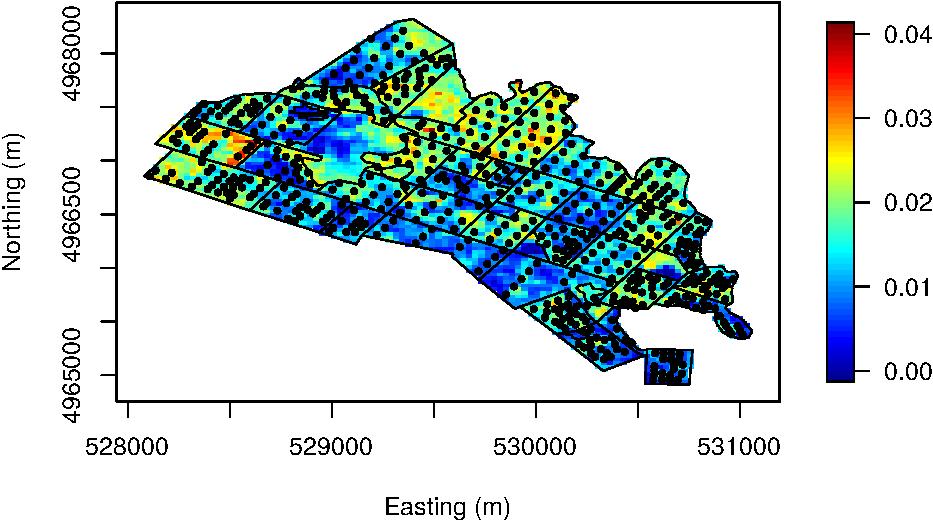
\includegraphics{bookdown_files/figure-latex/img1-1.pdf}
\caption{\label{fig:img1}Surface of LiDAR energy returns at 12 m above the
ground, forest inventory plot locations, and management unit boundaries
on the PEF.}
\end{figure}

\section{Zürichberg Forest inventory data set}\label{zf}

Measuring tree diameter and height is a time consuming process. This
fact makes the Zürichberg Forest inventory data set a rare and
impressive investment. These data comprise a complete enumeration of the
589 trees in the Zürichberg Forest, including species, diameter at
breast height, basal area, and volume. The stem map colored by species
is shown in Figure \ref{fig:zf}.

\begin{figure}
\centering
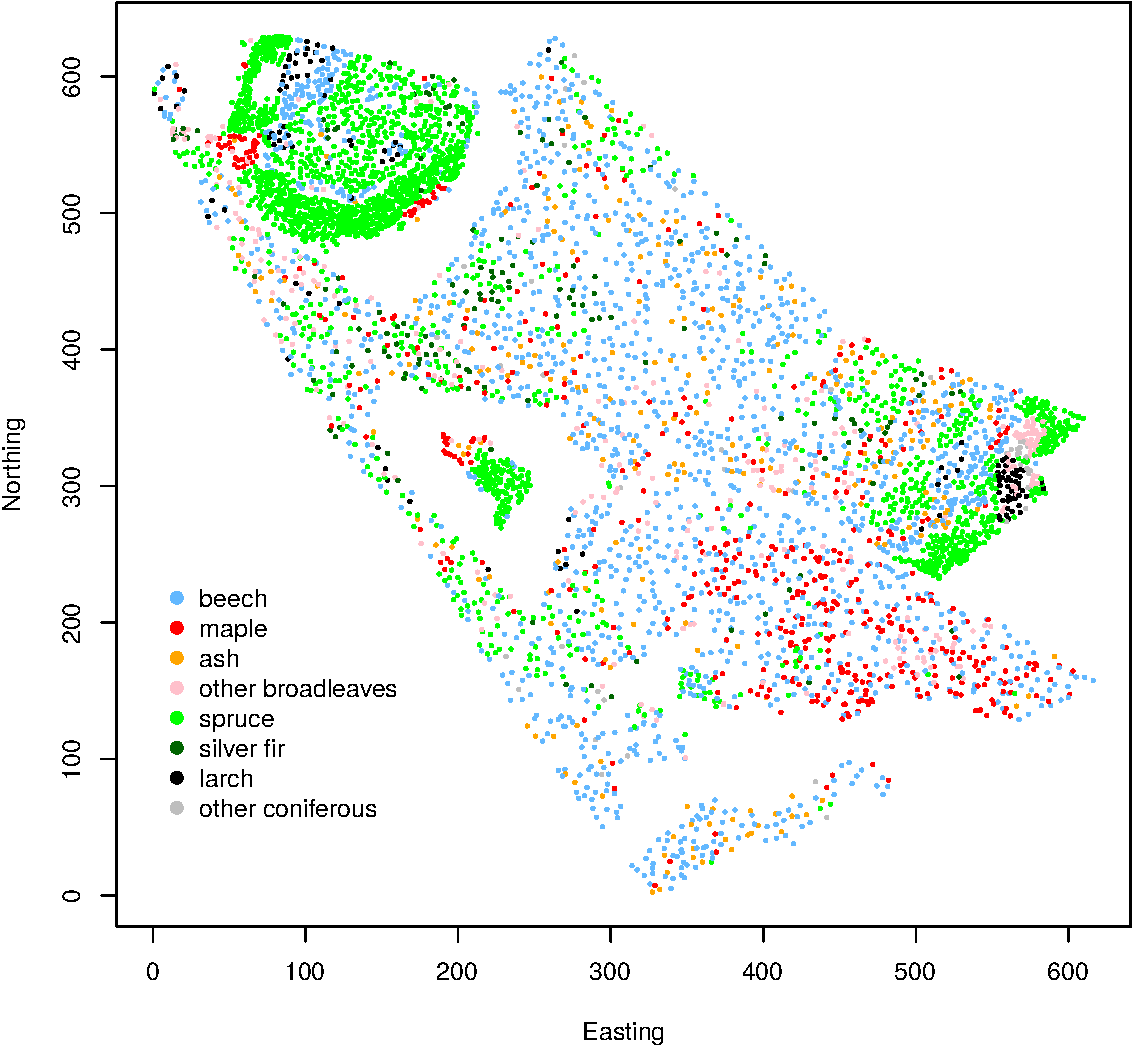
\includegraphics{bookdown_files/figure-latex/zf-1.pdf}
\caption{\label{fig:zf}Location and species of all trees in the Zürichberg
Forest.}
\end{figure}

\section{Looking Forward}\label{looking-forward}

The four examples above illustrate a variety of data sets that might be
encountered in practice, and each provides its own challenges. For the
FACE data, the challenges are more statistical in nature. Complications
could arise related to the complex study design and how that design
might affect methods of analysis and conclusions drawn from the study.
The other data sets present different challenges, such as how to:

\begin{enumerate}
\def\labelenumi{\arabic{enumi}.}
\tightlist
\item
  Develop biomass equations suitable for population inference from the
  FEF's small sample of 88 trees
\item
  Work with spatially indexed data in the case of the PEF and Zürichberg
  inventory data
\item
  Effectively and efficiently process the PEF's high-dimentional LiDAR
  signal data for use in predictive models of forest variables.
\end{enumerate}

This book and associated material introduce tools to tackle some of the
challenges in working with real data sets within the context of the R
statistical system. We will focus on important topics such as

\begin{itemize}
\tightlist
\item
  Obtaining and manipulating data
\item
  Summarizing and visualizing data
\item
  Communicating findings about data that support reproducible research
\item
  Programming and writing functions
\item
  Working with specialized data structures, e.g., spatial data and
  databases
\end{itemize}

\section{How to Learn (The Most Important Section in This
Book!)}\label{how-to-learn-the-most-important-section-in-this-book}

There are several ways to engage with the content of this book and
associated materials.

One way is not to engage at all. Leave the book closed on a shelf and do
something else with your time. That may or may not be a good life
strategy, depending on what else you do with your time, but you won't
learn much from the book!

Another way to engage is to read through the book ``passively'', reading
all that's written but not reading the book with R open on your
computer, where you could enter the R commands from the book. With this
strategy you'll probably learn more than if you leave the book closed on
a shelf, but there are better options.

A third way to engage is to read the book while you're at a computer
with R, and to enter the R commands from the book as you read about
them. You'll likely learn more this way.

A fourth strategy is even better. In addition to reading and entering
the commands given in the book, you think about what you're doing, and
ask yourself questions (which you then go on to answer). For example,
after working through some R code computing the logarithm of positive
numbers you might ask yourself, ``What would R do if I asked it to
calculate the logarithm of a negative number? What would R do if I asked
it to calculate the logarithm of a really large number such as one
trillion?'' You could explore these questions easily by just trying
things out in the R Console window.

If your goal is to maximize the time you have to binge-watch
\emph{Stranger Things} Season 2 on Netflix, the first strategy may be
optimal. But if your goal is to learn a lot about computational tools
for data science, the fourth strategy is probably going to be best.

\chapter{Introduction to R and
RStudio}\label{introduction-to-r-and-rstudio}

Various statistical and programming software environments are used in
data science, including R, Python, SAS, C++, SPSS, and many others. Each
has strengths and weaknesses, and often two or more are used in a single
project. This book focuses on R for several reasons:

\begin{enumerate}
\def\labelenumi{\arabic{enumi}.}
\tightlist
\item
  R is free
\item
  It is one of, if not the, most widely used software environments in
  data science
\item
  R is under constant and open development by a diverse and expert core
  group
\item
  It has an incredible variety of contributed packages
\item
  A new user can (relatively) quickly gain enough skills to obtain,
  manage, and analyze data in R
\end{enumerate}

Several enhanced interfaces for R have been developed. Generally such
interfaces are referred to as \emph{integrated development environments
(IDE)}. These interfaces are used to facilitate software development. At
minimum, an IDE typically consists of a source code editor and build
automation tools. We will use the RStudio IDE, which according to its
developers ``is a powerful productive user interface for R.\footnote{\url{http://www.rstudio.com/}}
RStudio is widely used, it is used increasingly in the R community, and
it makes learning to use R a bit simpler. Although we will use RStudio,
most of what is presented in this book can be accomplished in R (without
an added interface) with few or no changes.

\section{Obtaining and Installing R}\label{obtaining-and-installing-r}

It is simple to install R on computers running Microsoft Windows, macOS,
or Linux. For other operating systems users can compile the source code
directly.\footnote{Windows, macOS, and Linux users also can compile the
  source code directly, but for most it is a better idea to install R
  from already compiled binary distributions.} Here is a step-by-step
guide to installing R for Microsoft Windows.\footnote{New versions of R
  are released regularly, so the version number in Step 6 might be
  different from what is listed below.} macOS and Linux users would
follow similar steps.

\begin{enumerate}
\def\labelenumi{\arabic{enumi}.}
\tightlist
\item
  Go to \url{http://www.r-project.org/}
\item
  Click on the \texttt{CRAN} link on the left side of the page
\item
  Choose one of the mirrors.\footnote{The \url{http://cran.rstudio.com/}
    mirror is usually fast. Otherwise choose a mirror in Michigan.}
\item
  Click on \texttt{Download\ R\ for\ Windows}
\item
  Click on \texttt{base}
\item
  Click on \texttt{Download\ R\ 3.5.0\ for\ Windows}
\item
  Install R as you would install any other Windows program
\end{enumerate}

\section{Obtaining and Installing
RStudio}\label{obtaining-and-installing-rstudio}

You must install R prior to installing RStudio. RStudio is also simple
to install:

\begin{enumerate}
\def\labelenumi{\arabic{enumi}.}
\tightlist
\item
  Go to \url{http://www.rstudio.com}
\item
  Click on the link \texttt{RStudio} under the \texttt{Products} tab,
  then select the \texttt{Desktop} option
\item
  Click on the \texttt{Desktop} link
\item
  Choose the \texttt{DOWNLOAD\ RSTUDIO\ DESKTOP} link in the
  \texttt{Open\ Source\ Edition} column
\item
  On the ensuing page, click on the \texttt{Installer} version for your
  operating system, and once downloaded, install as you would any
  program
\end{enumerate}

\section{Using R and RStudio}\label{using-r-and-rstudio}

Start RStudio as you would any other program in your operating system.
For example, under Microsoft Windows use the Start Menu or double click
on the shortcut on the desktop (if a shortcut was created in the
installation process). A (rather small) view of RStudio is displayed in
Figure \ref{fig:rstudio}.

\begin{figure}
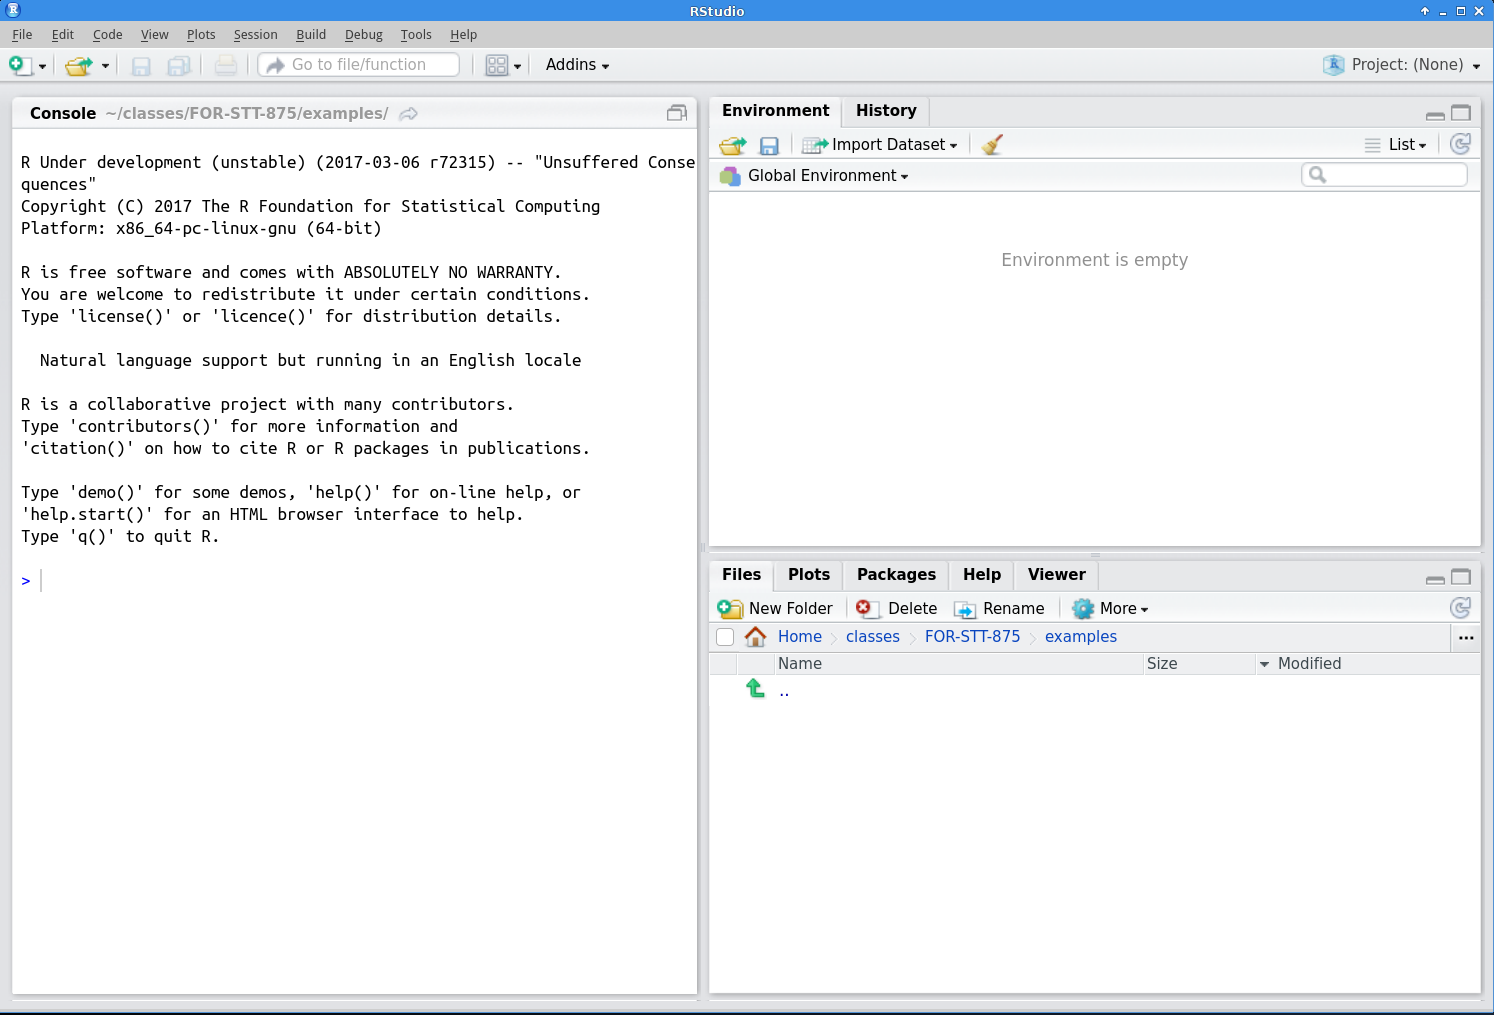
\includegraphics[width=20.75in]{02-introToR/02-images/RStudio} \caption{The Rstudio IDE.}\label{fig:rstudio}
\end{figure}

Initially the RStudio window contains three smaller windows. For now our
main focus will be the large window on the left, the \texttt{Console}
window, in which R statements are typed. The next few sections give
simple examples of the use of R. In these sections we will focus on
small and non-complex data sets, but of course later in the book we will
work with much larger and more complex sets of data. Read these sections
at your computer with R running, and enter the R commands there to get
comfortable using the R console window and RStudio.

\subsection{R as a calculator}\label{r-as-a-calculator}

R can be used as a calculator. Note that \texttt{\#} is the comment
character in R, so R ignores everything following this character. Also,
you will see that R prints \texttt{{[}1{]}} before the results of each
command. Soon we will explain its relevance, but ignore this for now.
The command prompt in R is the greater than sign
\texttt{\textgreater{}}.

\begin{Shaded}
\begin{Highlighting}[]
\OperatorTok{>}\StringTok{ }\DecValTok{34}\OperatorTok{+}\DecValTok{20}\OperatorTok{*}\KeywordTok{sqrt}\NormalTok{(}\DecValTok{100}\NormalTok{)  ## +,-,*,/ have the expected meanings}
\end{Highlighting}
\end{Shaded}

\begin{verbatim}
## [1] 234
\end{verbatim}

\begin{Shaded}
\begin{Highlighting}[]
\OperatorTok{>}\StringTok{ }\KeywordTok{exp}\NormalTok{(}\DecValTok{2}\NormalTok{)  ##The exponential function}
\end{Highlighting}
\end{Shaded}

\begin{verbatim}
## [1] 7.389
\end{verbatim}

\begin{Shaded}
\begin{Highlighting}[]
\OperatorTok{>}\StringTok{ }\KeywordTok{log10}\NormalTok{(}\DecValTok{100}\NormalTok{)  ##Base 10 logarithm}
\end{Highlighting}
\end{Shaded}

\begin{verbatim}
## [1] 2
\end{verbatim}

\begin{Shaded}
\begin{Highlighting}[]
\OperatorTok{>}\StringTok{ }\KeywordTok{log}\NormalTok{(}\DecValTok{100}\NormalTok{)  ##Base e logarithm}
\end{Highlighting}
\end{Shaded}

\begin{verbatim}
## [1] 4.605
\end{verbatim}

\begin{Shaded}
\begin{Highlighting}[]
\OperatorTok{>}\StringTok{ }\DecValTok{10}\OperatorTok{^}\KeywordTok{log10}\NormalTok{(}\DecValTok{55}\NormalTok{)}
\end{Highlighting}
\end{Shaded}

\begin{verbatim}
## [1] 55
\end{verbatim}

Most functions in R can be applied to vector arguments rather than
operating on a single argument at a time. A \emph{vector} is a data
structure that contains elements of the same data type (i.e.~integers).

\begin{Shaded}
\begin{Highlighting}[]
\OperatorTok{>}\StringTok{ }\DecValTok{1}\OperatorTok{:}\DecValTok{25}\NormalTok{ ##The integers from 1 to 25}
\end{Highlighting}
\end{Shaded}

\begin{verbatim}
##  [1]  1  2  3  4  5  6  7  8  9 10 11 12 13 14 15 16 17
## [18] 18 19 20 21 22 23 24 25
\end{verbatim}

\begin{Shaded}
\begin{Highlighting}[]
\OperatorTok{>}\StringTok{ }\KeywordTok{log}\NormalTok{(}\DecValTok{1}\OperatorTok{:}\DecValTok{25}\NormalTok{) ##The base e logarithm of these integers}
\end{Highlighting}
\end{Shaded}

\begin{verbatim}
##  [1] 0.0000 0.6931 1.0986 1.3863 1.6094 1.7918 1.9459
##  [8] 2.0794 2.1972 2.3026 2.3979 2.4849 2.5649 2.6391
## [15] 2.7081 2.7726 2.8332 2.8904 2.9444 2.9957 3.0445
## [22] 3.0910 3.1355 3.1781 3.2189
\end{verbatim}

\begin{Shaded}
\begin{Highlighting}[]
\OperatorTok{>}\StringTok{ }\DecValTok{1}\OperatorTok{:}\DecValTok{25}\OperatorTok{*}\DecValTok{1}\OperatorTok{:}\DecValTok{25}\NormalTok{ ##What will this produce?}
\end{Highlighting}
\end{Shaded}

\begin{verbatim}
##  [1]   1   4   9  16  25  36  49  64  81 100 121 144
## [13] 169 196 225 256 289 324 361 400 441 484 529 576
## [25] 625
\end{verbatim}

\begin{Shaded}
\begin{Highlighting}[]
\OperatorTok{>}\StringTok{ }\DecValTok{1}\OperatorTok{:}\DecValTok{25}\OperatorTok{*}\DecValTok{1}\OperatorTok{:}\DecValTok{5}\NormalTok{ ##What about this?}
\end{Highlighting}
\end{Shaded}

\begin{verbatim}
##  [1]   1   4   9  16  25   6  14  24  36  50  11  24
## [13]  39  56  75  16  34  54  76 100  21  44  69  96
## [25] 125
\end{verbatim}

\begin{Shaded}
\begin{Highlighting}[]
\OperatorTok{>}\StringTok{ }\KeywordTok{seq}\NormalTok{(}\DataTypeTok{from=}\DecValTok{0}\NormalTok{, }\DataTypeTok{to=}\DecValTok{1}\NormalTok{, }\DataTypeTok{by=}\FloatTok{0.1}\NormalTok{) ##A sequence of numbers from 0 to 1}
\end{Highlighting}
\end{Shaded}

\begin{verbatim}
##  [1] 0.0 0.1 0.2 0.3 0.4 0.5 0.6 0.7 0.8 0.9 1.0
\end{verbatim}

\begin{Shaded}
\begin{Highlighting}[]
\OperatorTok{>}\StringTok{ }\KeywordTok{exp}\NormalTok{(}\KeywordTok{seq}\NormalTok{(}\DataTypeTok{from=}\DecValTok{0}\NormalTok{, }\DataTypeTok{to=}\DecValTok{1}\NormalTok{, }\DataTypeTok{by=}\FloatTok{0.1}\NormalTok{)) ##What will this produce?}
\end{Highlighting}
\end{Shaded}

\begin{verbatim}
##  [1] 1.000 1.105 1.221 1.350 1.492 1.649 1.822 2.014
##  [9] 2.226 2.460 2.718
\end{verbatim}

Now the mysterious square bracketed numbers appearing next to the output
make sense. R puts the position of the beginning value on a line in
square brackets before the line of output. For example if the output has
40 values, and 15 values appear on each line, then the first line will
have \texttt{{[}1{]}} at the left, the second line will have
\texttt{{[}16{]}} to the left, and the third line will have
\texttt{{[}31{]}} to the left.

\subsection{Basic descriptive statistics and graphics in
R}\label{sec:dec}

Of course it is easy to compute basic descriptive statistics and to
produce standard graphical representations of data. For illustration
consider the first 14 observations of tree height and DBH (diameter at
breast height) from the FEF data set. We will begin by entering these
data ``by hand'' using the \texttt{c()} function, which concatenates its
arguments into a vector. For larger data sets we will clearly want an
alternative way to enter data.

A style note: R has two widely used methods of assignment: the left
arrow, which consists of a less than sign followed immediately by a
dash: \texttt{\textless{}-} and the equals sign: \texttt{=}. Much ink
has been used debating the relative merits of the two methods, and their
subtle differences. Many leading R style guides (e.g., the Google style
guide at \url{https://google.github.io/styleguide/Rguide.xml} and the
Bioconductor style guide at
\url{http://www.bioconductor.org/developers/how-to/coding-style/})
recommend the left arrow \texttt{\textless{}-} as an assignment
operator, and we will use this throughout the book.

Also you will see that if a command has not been completed but the ENTER
key is pressed, the command prompt changes to a \texttt{+} sign.

\begin{Shaded}
\begin{Highlighting}[]
\OperatorTok{>}\StringTok{ }\NormalTok{dbh <-}\StringTok{ }\KeywordTok{c}\NormalTok{(}\DecValTok{6}\NormalTok{, }\FloatTok{6.9}\NormalTok{, }\FloatTok{6.4}\NormalTok{, }\FloatTok{6.5}\NormalTok{, }\FloatTok{7.2}\NormalTok{, }\FloatTok{3.1}\NormalTok{, }\DecValTok{2}\NormalTok{, }\FloatTok{4.1}\NormalTok{, }\FloatTok{2.4}\NormalTok{, }\FloatTok{2.7}\NormalTok{, }\FloatTok{3.7}\NormalTok{, }\FloatTok{6.3}\NormalTok{, }\FloatTok{5.2}\NormalTok{, }\FloatTok{5.1}\NormalTok{, }\FloatTok{6.4}\NormalTok{)}
\OperatorTok{>}\StringTok{ }\NormalTok{ht <-}\StringTok{ }\KeywordTok{c}\NormalTok{(}\DecValTok{48}\NormalTok{, }\DecValTok{48}\NormalTok{, }\DecValTok{48}\NormalTok{, }\DecValTok{49}\NormalTok{, }\DecValTok{51}\NormalTok{, }\DecValTok{40}\NormalTok{, }\FloatTok{30.5}\NormalTok{, }\DecValTok{50}\NormalTok{, }\DecValTok{28}\NormalTok{, }\FloatTok{40.4}\NormalTok{, }\FloatTok{42.6}\NormalTok{, }\DecValTok{53}\NormalTok{, }\DecValTok{55}\NormalTok{, }\DecValTok{50}\NormalTok{, }\DecValTok{50}\NormalTok{)}
\OperatorTok{>}\StringTok{ }\NormalTok{dbh}
\end{Highlighting}
\end{Shaded}

\begin{verbatim}
##  [1] 6.0 6.9 6.4 6.5 7.2 3.1 2.0 4.1 2.4 2.7 3.7 6.3
## [13] 5.2 5.1 6.4
\end{verbatim}

\begin{Shaded}
\begin{Highlighting}[]
\OperatorTok{>}\StringTok{ }\NormalTok{ht}
\end{Highlighting}
\end{Shaded}

\begin{verbatim}
##  [1] 48.0 48.0 48.0 49.0 51.0 40.0 30.5 50.0 28.0 40.4
## [11] 42.6 53.0 55.0 50.0 50.0
\end{verbatim}

Next we compute some descriptive statistics for the two numeric
variables

\begin{Shaded}
\begin{Highlighting}[]
\OperatorTok{>}\StringTok{ }\KeywordTok{mean}\NormalTok{(dbh)}
\end{Highlighting}
\end{Shaded}

\begin{verbatim}
## [1] 4.933
\end{verbatim}

\begin{Shaded}
\begin{Highlighting}[]
\OperatorTok{>}\StringTok{ }\KeywordTok{sd}\NormalTok{(dbh)}
\end{Highlighting}
\end{Shaded}

\begin{verbatim}
## [1] 1.782
\end{verbatim}

\begin{Shaded}
\begin{Highlighting}[]
\OperatorTok{>}\StringTok{ }\KeywordTok{summary}\NormalTok{(dbh)}
\end{Highlighting}
\end{Shaded}

\begin{verbatim}
##    Min. 1st Qu.  Median    Mean 3rd Qu.    Max. 
##    2.00    3.40    5.20    4.93    6.40    7.20
\end{verbatim}

\begin{Shaded}
\begin{Highlighting}[]
\OperatorTok{>}\StringTok{ }\KeywordTok{mean}\NormalTok{(ht)}
\end{Highlighting}
\end{Shaded}

\begin{verbatim}
## [1] 45.57
\end{verbatim}

\begin{Shaded}
\begin{Highlighting}[]
\OperatorTok{>}\StringTok{ }\KeywordTok{sd}\NormalTok{(ht)}
\end{Highlighting}
\end{Shaded}

\begin{verbatim}
## [1] 7.857
\end{verbatim}

\begin{Shaded}
\begin{Highlighting}[]
\OperatorTok{>}\StringTok{ }\KeywordTok{summary}\NormalTok{(ht)}
\end{Highlighting}
\end{Shaded}

\begin{verbatim}
##    Min. 1st Qu.  Median    Mean 3rd Qu.    Max. 
##    28.0    41.5    48.0    45.6    50.0    55.0
\end{verbatim}

Next, a scatter plot of \texttt{dbh} versus \texttt{ht}:

\begin{Shaded}
\begin{Highlighting}[]
\KeywordTok{plot}\NormalTok{(dbh, ht)}
\end{Highlighting}
\end{Shaded}

\begin{center}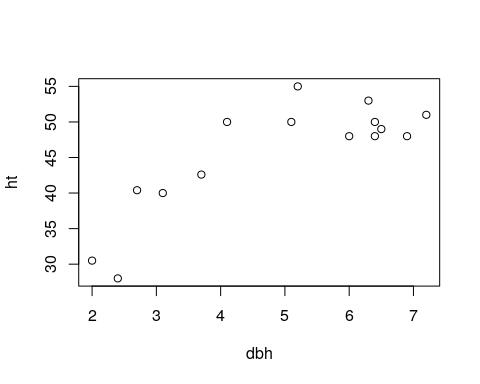
\includegraphics{bookdown_files/figure-latex/unnamed-chunk-4-1} \end{center}

Unsurprisingly as DBH increases, height tends to increase. We'll
investigate this further using simple linear regression in the next
section.

\subsection{Simple linear regression in
R}\label{simple-linear-regression-in-r}

The \texttt{lm()} function is used to fit linear models in R, including
simple linear regression models. Here it is applied to the DBH height
data.

\begin{Shaded}
\begin{Highlighting}[]
\OperatorTok{>}\StringTok{ }\NormalTok{ht.lm <-}\StringTok{ }\KeywordTok{lm}\NormalTok{(ht }\OperatorTok{~}\StringTok{ }\NormalTok{dbh) ##Fit the model and save it in ht.lm}
\OperatorTok{>}\StringTok{ }\KeywordTok{summary}\NormalTok{(ht.lm)  ##Basic summary of the model}
\end{Highlighting}
\end{Shaded}

\begin{verbatim}
## 
## Call:
## lm(formula = ht ~ dbh)
## 
## Residuals:
##    Min     1Q Median     3Q    Max 
## -8.507 -2.742 -0.812  2.683  8.480 
## 
## Coefficients:
##             Estimate Std. Error t value Pr(>|t|)    
## (Intercept)   27.925      3.739    7.47  4.7e-06 ***
## dbh            3.576      0.716    5.00  0.00024 ***
## ---
## Signif. codes:  
## 0 '***' 0.001 '**' 0.01 '*' 0.05 '.' 0.1 ' ' 1
## 
## Residual standard error: 4.77 on 13 degrees of freedom
## Multiple R-squared:  0.658,  Adjusted R-squared:  0.631 
## F-statistic:   25 on 1 and 13 DF,  p-value: 0.000244
\end{verbatim}

\begin{Shaded}
\begin{Highlighting}[]
\OperatorTok{>}\StringTok{ }\KeywordTok{plot}\NormalTok{(dbh, ht) ##Scatter plot of the data}
\OperatorTok{>}\StringTok{ }\KeywordTok{abline}\NormalTok{(ht.lm) ##Add the fitted regression line to the plot}
\end{Highlighting}
\end{Shaded}

\begin{center}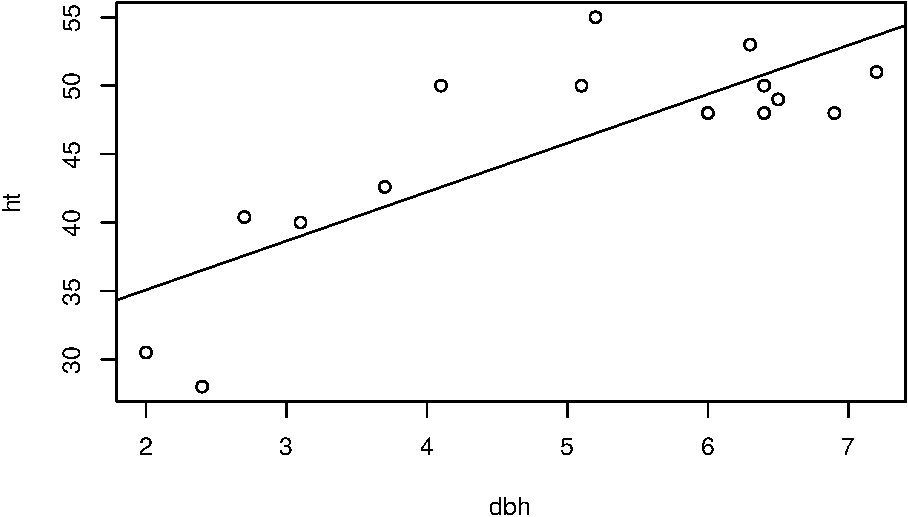
\includegraphics{bookdown_files/figure-latex/unnamed-chunk-5-1} \end{center}

We will work extensively with such models later in the text. We will
also talk about why it might not be a good idea to assume a linear
relationship between DBH and height---can you guess why this is by
looking at the data scatter and model fitted line in the plot above?

\section{How to Learn}\label{how-to-learn}

There are several ways to engage with the content of this book and
associated learning materials.

A comprehensive, but slightly overwhelming, cheatsheet for RStudio is
available here
\url{https://www.rstudio.com/wp-content/uploads/2016/01/rstudio-IDE-cheatsheet.pdf}.
As we progress in learning R and RStudio, this cheatsheet will become
more useful. For now you might use the cheatsheet to locate the various
windows and functions identified in the coming chapters.

\section{Getting help}\label{getting-help}

There are several free (and several not free) ways to get R help when
needed.

Several help-related functions are built into R. If there's a particular
R function of interest, such as \texttt{log}, \texttt{help(log)} or
\texttt{?log} will bring up a help page for that function. In RStudio
the help page is displayed, by default, in the \texttt{Help} tab in the
lower right window.\footnote{There are ways to change this default
  behavior.} The function \texttt{help.start} opens a window which
allows browsing of the online documentation included with R. To use
this, type \texttt{help.start()} in the console window.\footnote{You may
  wonder about the parentheses after \texttt{help.start}. A user can
  specify arguments to any R function inside parentheses. For example
  \texttt{log(10)} asks R to return the logarithm of the argument 10.
  Even if no arguments are needed, R requires empty parentheses at the
  end of any function name. In fact if you just type the function name
  without parentheses, R returns the definition of the function. For
  simple functions this can be illuminating.} The \texttt{help.start}
function also provides several manuals online and can be a useful
interface in addition to the built in help.

Search engines provide another, sometimes more user-friendly, way to
receive answers for R questions. A Google search often quickly finds
something written by another user who had the same (or a similar)
question, or an online tutorial that touches on the question. More
specialized is \url{https://rseek.org/}, which is a search engine
focused specifically on R. Both Google and \url{https://rseek.org} are
valuable tools, often providing more user-friendly information then R's
own help system.

In addition, R users have written many types of contributed
documentation. Some of this documentation is available at
\url{http://cran.r-project.org/other-docs.html}. Of course there are
also numerous books covering general and specialized R topics available
for purchase.

\section{Workspace, working directory, and keeping
organized}\label{workspace-working-directory-and-keeping-organized}

The \emph{workspace} is your R session working environment and includes
any objects you create. Recall these objects are listed in the
\texttt{Global\ Environment} window. The command \texttt{ls()}, which
stands for list, will also list all the objects in your workspace (note,
this is the same list that is given in the \texttt{Global\ Environment}
window). When you close RStudio, a dialog box will ask you if you want
to save an image of the current workspace. If you choose to save your
workspace, RStudio saves your session objects and information in a
\texttt{.RData} file (the period makes it a hidden file) in your
\emph{working directory}. Next time you start R or RStudio it checks if
there is a \texttt{.RData} in the working directory, loads it if it
exists, and your session continues where you left off. Otherwise R
starts with an empty workspace. This leads to the next question---what
is a working directory?

Each R session is associated with a working directory. This is just a
directory from which R reads and writes files, e.g., the \texttt{.RData}
file, data files you want to analyze, or files you want to save. On Mac
when you start RStudio it sets the working directory to your home
directory (for me that's \texttt{/Users/andy}). If you're on a different
operating system, you can check where the default working directory is
by typing \texttt{getwd()} in the console. You can change the default
working directory under RStudio's \texttt{Global\ Option} dialog found
under the \texttt{Tools} dropdown menu. There are multiple ways to
change the working directory once an R session is started in RStudio.
One method is to click on the \texttt{Files} tab in the lower right
window and then click the \texttt{More} button. Alternatively, you can
set the session's working directory using the \texttt{setwd()} in the
console. For example, on Windows
\texttt{setwd("C:/Users/andy/for472/exercise1")} will set the working
directory to \texttt{C:/Users/andy/for472/exercise1}, assuming that file
path and directory exist (Note: Windows file path uses a backslash,
\texttt{\textbackslash{}}, but in R the backslash is an escape
character, hence specifying file paths in R on Windows uses the forward
slash, i.e., \texttt{/}). Similarly on Mac you can use
\texttt{setwd("/Users/andy/for472/exercise1")}. Perhaps the most simple
method is to click on the \texttt{Session} tab at the top of your screen
and click on the \texttt{Set\ Working\ Directory} option. Later on when
we start reading and writing data from our R session, it will be very
important that you are able to identify your current working directory
and change it if needed. We will revisit this in subsequent chapters.

As with all work, keeping organized is the key to efficiency. It is good
practice to have a dedicated directory for each R project or exercise.

\section{Quality of R code}\label{quality-of-r-code}

\begin{figure}
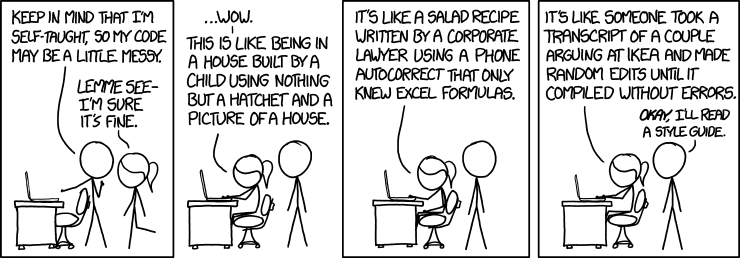
\includegraphics[width=10.28in]{02-introToR/02-images/code_quality} \caption{xkcd: Code Quality}\label{fig:comic}
\end{figure}

Writing well-organized and well-labeled code allows your code to be more
easily read and understood by another person. (See xkcd's take on code
quality in Figure \ref{fig:comic}.) More importantly, though, your
well-written code is more accessible to you hours, days, or even months
later. We are hoping that you can use the code you write in this class
in future projects and research.

Google provides style guides for many programming languages. You can
find the R style guide
\href{https://google.github.io/styleguide/Rguide.xml}{here}. Below are a
few of the key points from the guide that we will use right away.

\subsection{Naming Files}\label{naming-files}

File names should be meaningful and end in \texttt{.R}. If we write a
script that analyzes a certain species distribution:

\begin{itemize}
\tightlist
\item
  GOOD: \(\color{green}{\verb+african_rhino_distribution.R+}\)
\item
  GOOD: \(\color{green}{\verb+africanRhinoDistribution.R+}\)
\item
  BAD: \(\color{red}{\verb+speciesDist.R+}\) (too ambiguous)
\item
  BAD: \(\color{red}{\verb+species.dist.R+}\) (too ambiguous and two
  periods can confuse operating systems' file type auto-detect)
\item
  BAD: \(\color{red}{\verb+speciesdist.R+}\) (too ambiguous and
  confusing)
\end{itemize}

\subsection{Naming Variables}\label{naming-variables}

\begin{itemize}
\tightlist
\item
  GOOD: \(\color{green}{\verb+rhino.count+}\)
\item
  GOOD: \(\color{green}{\verb+rhinoCount+}\)
\item
  GOOD: \(\color{green}{\verb+rhino_count+}\) (We don't mind the
  underscore and use it quite often, although Google's style guide says
  it's a no-no for some reason)
\item
  BAD: \(\color{red}{\verb+rhinocount+}\) (confusing)
\end{itemize}

\subsection{Syntax}\label{syntax}

\begin{itemize}
\tightlist
\item
  Keep code lines under 80 characters long.
\item
  Indent your code with two spaces. (RStudio does this by default when
  you press the TAB key.)
\end{itemize}

\chapter{Scripts, R Markdown, and Reproducible
Research}\label{scripts-r-markdown-and-reproducible-research}

Doing work in data science, whether for homework, a project for a
business, or a research project, typically involves several iterations.
For example creating an effective graphical representation of data can
involve trying out several different graphical representations, and then
tens if not hundreds of iterations when fine-tuning the chosen
representation. And each of these representations may require several R
commands to create. Although this all could be accomplished by typing
and re-typing commands at the R Console, it is easier and more effective
to write the commands in a \texttt{script\ file} that can then be
submitted to the R console either a line at a time or all
together.\footnote{Unsurprisingly it is also possible to submit several
  selected lines of code at once.}

In addition to making the workflow more efficient, R scripts provide
another large benefit. Often we work on one part of a homework
assignment or project for a few hours, then move on to something else,
and then return to the original part a few days, months, or sometimes
even years later. In such cases we may have forgotten how we created a
graphical display that we were so proud of, and will again need to spend
a few hours to recreate it. If we save a script file, we have the
ingredients immediately available when we return to a portion of a
project.\footnote{In principle the R history mechanism provides a
  similar record. But with history we have to search through a lot of
  other code to find what we're looking for, and scripts are a much
  cleaner mechanism to record our work.}

Next consider a larger scientific endeavor. Ideally a scientific study
will be reproducible, meaning that an independent group of researchers
(or the original researchers) will able to duplicate the study. Thinking
about data science, this means that all the steps taken when working
with the data from a study should be reproducible, from selection of
variables to formal data analysis. In principle this can be facilitated
by explaining, in words, each step of the work with data. In practice,
on the other hand, it is typically difficult or impossible to reproduce
a full data analysis based on a written explanation. It is much more
effective to include the actual computer code which accomplished the
data work in the report, whether the report is a homework assignment or
a research paper. Tools in R such as \texttt{R\ Markdown} facilitate
this process.

\section{Scripts in R}\label{scripts-in-r}

As noted above, scripts help to make working with data more efficient
and provide a record of how data were managed and analyzed. Here we
describe an example using the FEF data.\footnote{The example uses
  features of R that we have not yet discussed, so don't worry about the
  details but rather about how it motivates the use of a script file.}
First we read the FEF data into R using the code below.

\begin{Shaded}
\begin{Highlighting}[]
\OperatorTok{>}\StringTok{ }\NormalTok{face.dat <-}\StringTok{ }\KeywordTok{read.csv}\NormalTok{(}
\OperatorTok{+}\StringTok{     }\DataTypeTok{file=}\StringTok{"http://blue.for.msu.edu/FOR472/data/FACE_aspen_core_growth.csv"}
\OperatorTok{+}\StringTok{ }\NormalTok{)}
\end{Highlighting}
\end{Shaded}

Next we print the names of the variables in the data set. Don't be
concerned about the specific details. Later we will learn much more
about reading in data and working with data sets in R.

\begin{Shaded}
\begin{Highlighting}[]
\OperatorTok{>}\StringTok{ }\KeywordTok{names}\NormalTok{(face.dat)}
\end{Highlighting}
\end{Shaded}

\begin{verbatim}
##  [1] "Rep"                 "Treat"              
##  [3] "Clone"               "E.Clone"            
##  [5] "Row"                 "Col"                
##  [7] "ID.."                "X1997Initial_Height"
##  [9] "X1997Initial_Diam"   "X1997Final_Height"  
## [11] "X1997Final_Diam"     "X1998_Height"       
## [13] "X1998_Diam"          "X1999_Height"       
## [15] "X1999_Diam"          "X2000_Height"       
## [17] "X2000_Diam"          "X2001_Height"       
## [19] "X2001_AvgDiam"       "X2001_Diam.3cm"     
## [21] "X2001_Diam.10cm"     "X2002_Height"       
## [23] "X2002_Diam.10cm"     "X2003_Height"       
## [25] "X2003_Diam.10cm"     "X2003_DBH"          
## [27] "X2004_Height"        "X2004_Diam.10cm"    
## [29] "X2004_DBH"           "X2005_Height"       
## [31] "X2005_Diam.10cm"     "X2005_DBH"          
## [33] "X2006_Height"        "X2006_DBH"          
## [35] "X2007_Height"        "X2007_DBH"          
## [37] "X2008_Height"        "X2008_DBH"          
## [39] "Notes"               "Comment1"           
## [41] "Comment2"            "Comment3"           
## [43] "Comment4"            "Comment5"           
## [45] "Comment6"
\end{verbatim}

Let's create a scatter plot of 2008 DBH versus height. To do this we'll
first create variables for DBH and height taken in the year 2008 and
print out the first ten values of each variable.\footnote{Neither of
  these steps are necessary, but are convenient for illustration.}

\begin{Shaded}
\begin{Highlighting}[]
\OperatorTok{>}\StringTok{ }\NormalTok{dbh <-}\StringTok{ }\NormalTok{face.dat}\OperatorTok{$}\NormalTok{X2008_DBH}
\OperatorTok{>}\StringTok{ }\NormalTok{ht <-}\StringTok{ }\NormalTok{face.dat}\OperatorTok{$}\NormalTok{X2008_Height}
\OperatorTok{>}\StringTok{ }\NormalTok{dbh[}\DecValTok{1}\OperatorTok{:}\DecValTok{10}\NormalTok{]}
\end{Highlighting}
\end{Shaded}

\begin{verbatim}
##  [1]   NA 9.55 2.00 9.00 3.11 6.35 4.60   NA   NA 1.42
\end{verbatim}

\begin{Shaded}
\begin{Highlighting}[]
\OperatorTok{>}\StringTok{ }\NormalTok{ht[}\DecValTok{1}\OperatorTok{:}\DecValTok{10}\NormalTok{]}
\end{Highlighting}
\end{Shaded}

\begin{verbatim}
##  [1]   NA 1225  334 1079  370  859  818   NA   NA  268
\end{verbatim}

The \texttt{NA} is how missing data are represented in R. Their presence
here suggests several trees in this data set are dead or not measured
for some reason in 2008. Of course at some point it would be good to
investigate which trees have missing data and why. The \texttt{plot()}
function in R will omit missing values, and for now we will just plot
the non-missing data. A scatter plot of the data is drawn next.

\begin{Shaded}
\begin{Highlighting}[]
\OperatorTok{>}\StringTok{ }\KeywordTok{plot}\NormalTok{(dbh, ht)}
\end{Highlighting}
\end{Shaded}

\begin{center}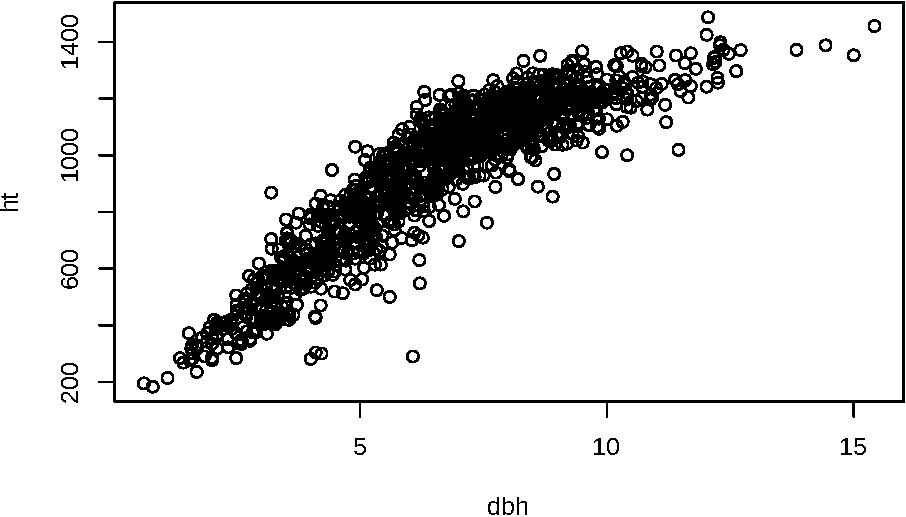
\includegraphics{bookdown_files/figure-latex/unnamed-chunk-9-1} \end{center}

Not surprisingly, the scatter plot shows that DBH and height are
positively correlated and the relationship is nonlinear. Now that we
have a basic scatter plot, it is tempting to make it more informative.
We will do this by adding a feature that identifies which trees belong
to the control and elevated CO\(_2\) environment treatments. We do this
by first separating DBH and height into their respective treatment
groups.

\begin{Shaded}
\begin{Highlighting}[]
\OperatorTok{>}\StringTok{ }\NormalTok{treat <-}\StringTok{ }\NormalTok{face.dat}\OperatorTok{$}\NormalTok{Treat}
\OperatorTok{>}\StringTok{ }\NormalTok{dbh.treat.}\DecValTok{1}\NormalTok{ <-}\StringTok{ }\NormalTok{dbh[treat}\OperatorTok{==}\DecValTok{1}\NormalTok{] ##Treatment 1 is the control}
\OperatorTok{>}\StringTok{ }\NormalTok{ht.treat.}\DecValTok{1}\NormalTok{ <-}\StringTok{ }\NormalTok{ht[treat}\OperatorTok{==}\DecValTok{1}\NormalTok{]}
\OperatorTok{>}\StringTok{ }
\ErrorTok{>}\StringTok{ }\NormalTok{dbh.treat.}\DecValTok{2}\NormalTok{ <-}\StringTok{ }\NormalTok{dbh[treat}\OperatorTok{==}\DecValTok{2}\NormalTok{] ##Treatment 2 is the elevated CO2}
\OperatorTok{>}\StringTok{ }\NormalTok{ht.treat.}\DecValTok{2}\NormalTok{ <-}\StringTok{ }\NormalTok{ht[treat}\OperatorTok{==}\DecValTok{2}\NormalTok{]}
\end{Highlighting}
\end{Shaded}

To make a more informative scatter plot we will do two things. First
make a plot for treatment 1 data, but ensure the plot region is large
enough to include the treatment 2 data. This is done by specifying the
range of the plot axes via \texttt{xlim} and \texttt{ylim} arguments in
the \texttt{plot()} function. Here the \texttt{xlim} and \texttt{ylim}
are set to the range of \texttt{dbh} and \texttt{ht} values,
respectively, using \texttt{range()} (try and figure out what the
\texttt{na.rm} argument does in the range function). Second we add
treatment 2 data via the \texttt{points()} function. There are several
other arguments passed to the plot function, but don't worry about these
detail for now.

\begin{Shaded}
\begin{Highlighting}[]
\OperatorTok{>}\StringTok{ }\KeywordTok{plot}\NormalTok{(dbh.treat.}\DecValTok{1}\NormalTok{, ht.treat.}\DecValTok{1}\NormalTok{, }\DataTypeTok{xlim=}\KeywordTok{range}\NormalTok{(dbh, }\DataTypeTok{na.rm=}\OtherTok{TRUE}\NormalTok{), }\DataTypeTok{ylim=}\KeywordTok{range}\NormalTok{(ht, }\DataTypeTok{na.rm=}\OtherTok{TRUE}\NormalTok{),}
\OperatorTok{+}\StringTok{      }\DataTypeTok{pch=}\DecValTok{19}\NormalTok{, }\DataTypeTok{col=}\StringTok{"salmon3"}\NormalTok{, }\DataTypeTok{cex=}\FloatTok{0.5}\NormalTok{, }\DataTypeTok{xlab=}\StringTok{"DBH (cm)"}\NormalTok{, }\DataTypeTok{ylab=}\StringTok{"Height (cm)"}\NormalTok{)}
\OperatorTok{>}\StringTok{ }\KeywordTok{points}\NormalTok{(dbh.treat.}\DecValTok{2}\NormalTok{, ht.treat.}\DecValTok{2}\NormalTok{, }\DataTypeTok{pch=}\DecValTok{19}\NormalTok{, }\DataTypeTok{col=}\StringTok{"blue"}\NormalTok{, }\DataTypeTok{cex=}\FloatTok{0.5}\NormalTok{)}
\end{Highlighting}
\end{Shaded}

\begin{center}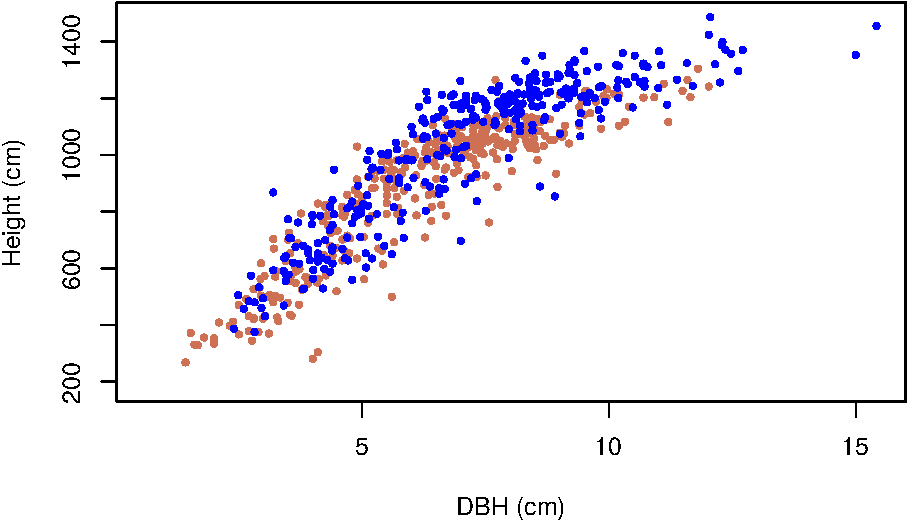
\includegraphics{bookdown_files/figure-latex/unnamed-chunk-11-1} \end{center}

Of course we should have a plot legend to tell the viewer which colors
are associated with treatments and a lot of other aesthetic refinements.
For now, however, we will resist such temptations.\footnote{As an aside,
  by only looking at the plotted data and thinking about basic plant
  physiology, can you guess which color is associated with the elevated
  CO\(_2\) treatment?}

Some of the process leading to the completed plot is shown above. We
read in the data, created an intermediate plot by adding treatment
identifiers, creating variables representing the 2008 measurements of
DBH and height, and so on. A lot of the process isn't shown, to save
space. For example, I made several mistakes in the process of getting
the code and plot the way I wanted it---forgot the \texttt{na.rm=TRUE}
initially then fiddled around with the treatment colors a bit.

Now imagine trying to recreate the plot a few days later. Possibly
someone saw the plot and commented that it would be interesting to see
similar plots for each year in the study period. If all the work,
including all the false starts and refinements, were done at the
console, it would be hard to sort things out and would take longer than
necessary to create the new plots. This would be especially true if a
few months had passed, rather than just a few days.

Creating the new scatter plots would be much easier with a script file,
especially if it had a few well-chosen comments. Fortunately it is quite
easy to create and work with script files in RStudio.\footnote{It is
  also easy in R without RStudio. Just use
  \texttt{File\ \$\textgreater{}\$\ New\ script} to create a script
  file, and save it before exiting R.} Just choose
\texttt{File\ \$\textgreater{}\$\ New\ File\ \$\textgreater{}\$\ New\ script}
and a script window will open up in the upper left of the full RStudio
window.

An example of a script window (with some R code already typed in) is
shown in Figure \ref{fig:script}. From the script window the user can,
among other things, save the script (either using the \texttt{File} menu
or the icon near the top left of the window) and can run one or more
lines of code from the window (using the \texttt{run} icon in the
window, or by copying and pasting into the console window). In addition,
there is a \texttt{Source\ on\ Save} checkbox. If this is checked, the R
code in the script window is automatically read into R and executed when
the script file is saved.

\begin{figure}

{\centering 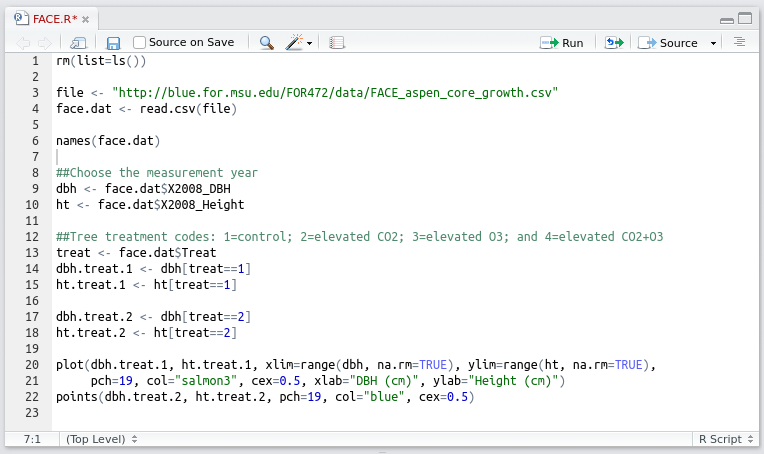
\includegraphics[width=10.61in]{03-scripts/03-images/FACE-script-screenshot} 

}

\caption{A script window in RStudio}\label{fig:script}
\end{figure}

\section{R Markdown}\label{r-markdown}

People typically work on data with a larger purpose in mind. Possibly
the purpose is to understand a biological system more clearly. Possibly
the purpose is to refine a system that recommends movies to users in an
online streaming movie service. Possibly the purpose is to complete a
homework assignment and demonstrate to the instructor an understanding
of an aspect of data analysis. Whatever the purpose, a key aspect is
communicating with the desired audience, for example, fellow researchers
or an instructor.

One possibility, which is somewhat effective, is to write a document
using software such as Microsoft Word \footnote{Or possibly \(\LaTeX\)
  if the document is more technical} and to include R output such as
computations and graphics by cutting and pasting into the main document.
One drawback to this approach is similar to what makes script files so
useful: If the document must be revised it may be hard to unearth the R
code that created graphics or analyses, to revise these.\footnote{Organizing
  the R code using script files and keeping all the work organized in a
  well-thought-out directory structure can help here, but this requires
  a level of forethought and organization that most people do not
  possess\(\ldots\)including myself.} A more subtle but possibly more
important drawback is that the reader of the document will not know
precisely how analyses were done, or how graphics were created. Over
time even the author(s) of the paper will forget the details. A verbal
description in a ``methods'' section of a paper can help here, but
typically these do not provide all the details of the analysis, but
rather might state something like, ``All analyses were carried out using
R version 3.3.1.''

RStudio's website provides an excellent overview of R Markdown
capabilities for reproducible research. At minimum, follow the
\texttt{Get\ Started} link at \url{http://rmarkdown.rstudio.com/} and
watch the introduction video.

Among other things, R Markdown provides a way to include R code that
read in data, create graphics, or perform analyses, all in a single
document that is processed to create a research paper, homework
assignment, or other written product. The R Markdown file is a plain
text file containing text the author wants to have show in the final
document, simple commands to indicate how the text should be formatted
(for example boldface or italic, or a bulleted list), and R code that
creates output (including graphics) on the fly. Perhaps the simplest way
to get started is to see an R Markdown file and the resulting document
that is produced after the R Markdown document is processed. Bewlo we
show a very simple R Markdown file, and Figure @ref\{fig:rmdout\} shows
the resulting output. In this case the output created is an HTML file,
but there are other possible output formats, such as Microsoft Word or
PDF.

\begin{verbatim}
---
title: "R Markdown"
author: "Andy Finley"
date: "April 3, 2017"
output: html_document
---

Basic formatting: 

*italic* 

**bold**

~~strikethrough~~ 

A code chunk:


```r
x <- 1:10
y <- 10:1
mean(x)
```

```
## [1] 5.5
```

```r
sd(y)
```

```
## [1] 3.028
```

Inline code:

10

Inline code not executed:

`5+5`
\end{verbatim}

\begin{figure}

{\centering 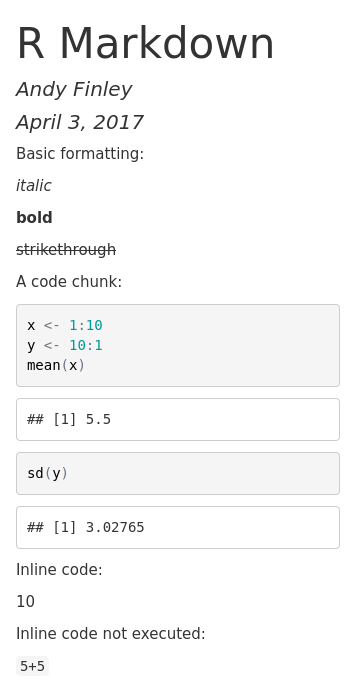
\includegraphics[width=4.9in]{03-scripts/03-images/Small-2} 

}

\caption{The R Markdown file that produces the output of the above code}\label{fig:rmdout}
\end{figure}

At the top of the input R Markdown file are some lines with
\texttt{-\/-\/-} at the top and the bottom. These lines are not needed,
but give a convenient way to specify the title, author, and date of the
article that are then typeset prominently at the top of the output
document. For now, don't be concerned with the lines following
\texttt{output:}. These can be omitted (or included as shown).

Next are a few lines showing some of the ways that font effects such as
italics, boldface, and strikethrough can be achieved. For example, an
asterisk before and after text sets the text in \emph{italics}, and two
asterisks before and after text sets the text in \textbf{boldface}.

More important for our purposes is the ability to include R code in the
R Markdown file, which will be executed with the output appearing in the
output document. Bits of R code included this way are called \emph{code
chunks}. The beginning of a code chunk is indicated with three backticks
and an ``r''" in curly braces. The end of a code chunk is indicated with
three backticks. For example, the R Markdown file in Figure
@ref(fig:rmd\_in) has one code chunk:

\begin{Shaded}
\begin{Highlighting}[]
\StringTok{```}\DataTypeTok{\{r\}}
\DataTypeTok{x = 1:10}
\DataTypeTok{y = 10:1}
\DataTypeTok{mean(x)}
\DataTypeTok{sd(y)}
\StringTok{```}
\end{Highlighting}
\end{Shaded}

In this code chunk two vectors \texttt{x} and \texttt{y} are created,
and the mean of \texttt{x} and the standard deviation of \texttt{y} are
computed. In the output in Figure @ref(fig:rmd\_out) the R code is
reproduced, and the output of the two lines of code asking for the mean
and standard deviation is shown.

\chapter*{References}\label{references}


\bibliography{text.bib}

\backmatter
\printindex

\end{document}
